\documentclass[11pt]{article}
\usepackage{amsmath, amssymb, amsfonts,  graphicx, enumerate, float, wrapfig, hyperref}
\usepackage[margin=0.5in]{geometry}
\graphicspath{{./}}
\newcommand*{\vs}{\vspace{1cm}}
\newcommand*{\next}{\noindent}
\newcommand*{\set}{\setcounter{equation}{0}}

\begin{document}

\title{3.6 A Summary of Curve Sketching}
\author{Juan J. Moreno Santos}
\date{November 2023}

\maketitle
\section{Match the graph of $f$ in the left column with that of its derivative in the right column.}
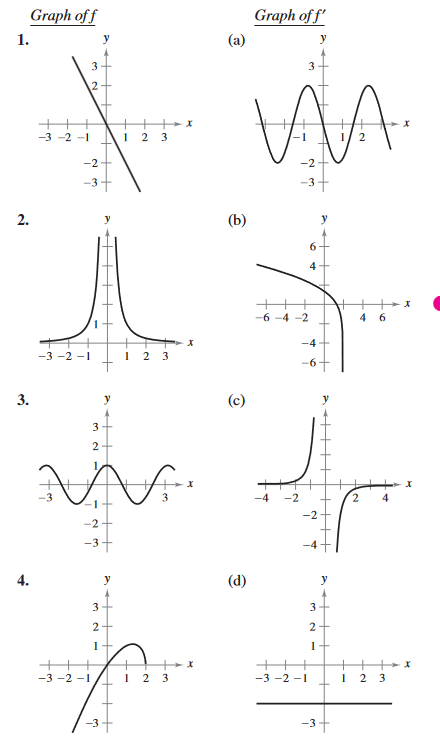
\includegraphics[scale=0.8]{2.png}\\
2. As $x$ goes to zero from the left, $f$'s slope approaches $\infty$. Likewise, $f$'s slope approaches $-\infty$ as x approaches zero from the right. Therefore, its derivative is (c).

\vs\next
4. The slope of the graph is positive up to $x\approx 1.5$; therefore, the function's derivative is (b).

\section{Analyze and sketch a graph of the function. Label any intercepts, relative extrema, points of inflection, and asymptotes. Use a graphing utility to verify your results.}
8.\[\frac{x^2+1}{x^2-4}\]
\begin{align}
    y'&=\frac{-10x}(x^2-4)^2=0\,\,\text{when}\,\, x=0\\
    y''&=\frac{10(3x^2+4)}{(x^2-4)^3}<0\,\,\text{when}\,\, x=0
\end{align}
\begin{enumerate}
    \item Relative maxima: $(0, -\frac{1}{4})$
    \item Intercepts: $(0, -\frac{1}{4})$
    \item Symmetric in the y-axis
    \item Vertical asymptotes: $x=\pm 2$
    \item Horizontal asymptotes: $y=1$
\end{enumerate}
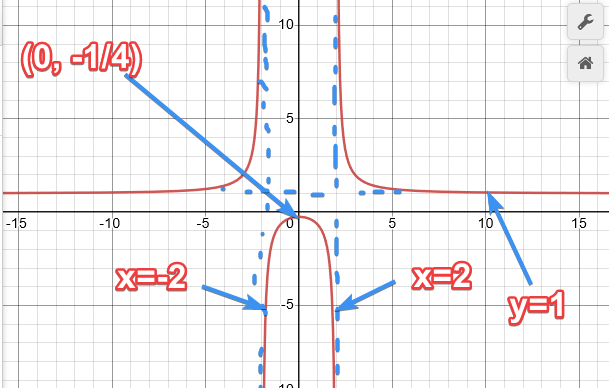
\includegraphics{8.png}

\vs\next
16.\begin{align}
    \set
y&=\frac{2x^2-5x+5}{x-2}=2x-1+\frac{3}{x-2}\\
y'&=2-\frac{3}{(x-2)^2}=\frac{2x^2-8x+5}{(x-2)^2}=0\,\,\text{when}\,\, x=\frac{4\pm\sqrt[]{6}}{2}\\
y ''&=\frac{6}{(x-2)^3}\neq 0
\end{align}
\begin{enumerate}
    \item Relative maxima: $\left(\frac{4-\sqrt[]{6}}{2},\,\,-1.8990\right)$
    \item Relative minima: $\left(\frac{4+\sqrt[]{6}}{2},\,\,7,8990\right)$
    \item Intercept: $(0, -\frac{5}{2})$
    \item Vertical asymptotes: $x=2$
    \item Slant asymptotes: $y=2x-1$
\end{enumerate}
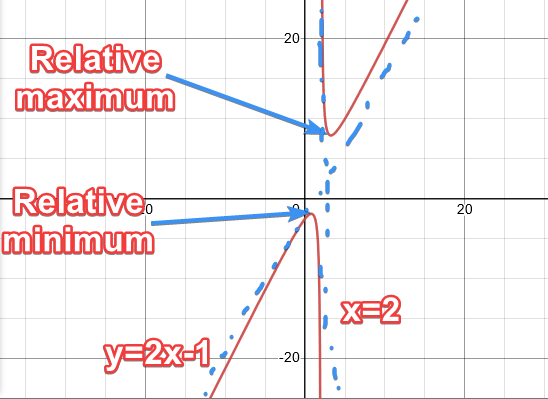
\includegraphics{16.png}

\vs\next
24.\begin{align}
    \set
    y&=-\frac{1}{3}(x^3-3x+2)\\
    y'&=-x^2+1=-\,\,\text{when}\,\, x=\pm 1\\
    y''&=-2x=0\,\,\text{when}\,\, x=0
\end{align}
\begin{flushleft}
    \begin{table}[h]
        \begin{tabular}{|l|l|l|l|l|}
        \hline
         & $y$ & $y'$ & $y''$ & Conclusion\\\hline
         $-\infty<x<-1$ & & - & + & Decreasing and concave up\\\hline
         $x=-1$ & $-\frac{4}{3}$ & 0 & + & Relative minimum\\\hline
         $-1<x<0$ & & + & + & Increasing and concave up\\\hline
         $x=0$ & $-\frac{2}{3}$ & + & 0 & Point of inflection\\\hline
         $0<x<1$ & & + & - & Increasing and concave down\\\hline
         $x=1$ & 0 & 0 & - & Relative maximum\\\hline
         $1<x<\infty$ & & - & - & Decreasing and concave down\\\hline
        \end{tabular}
    \end{table}
\end{flushleft}
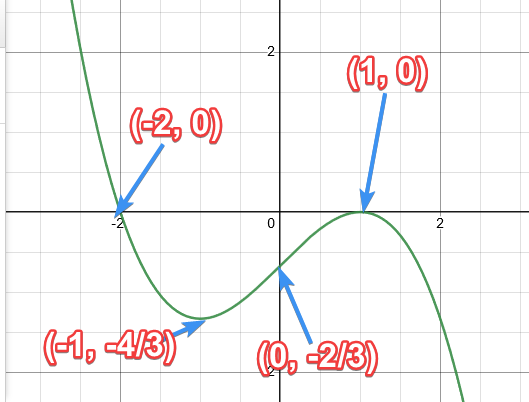
\includegraphics{24.png}

\section{Sketch a graph of the function over the given interval. Use a graphing utility to verify your graph.}
28.\begin{align}
    \set
    f(x)&=-x+2\cos x,\,\,0\leq x\leq 2\pi\\
    f'(x)&=-1-2\sin x\\
    f''(x)&=-2\cos x\\
    f(x)&=0\,\,\text{at}\,\, x\approx 1.03\\
    f'(x)&=0\Rightarrow\sin x=-\frac{1}{2}\Rightarrow x=\frac{7\pi}{6},\,\,\frac{11\pi}{6}\\
    f''(x)&=0\Rightarrow x=\frac{\pi}{2},\,\,\frac{3\pi}{2}
\end{align}
\begin{enumerate}
    \item Relative minimum: $\left(\frac{7\pi}{6},\,\,-\sqrt[]{3}-\frac{7\pi}{6}\right)\approx\left(3.665,\,\,-5.397\right)$
    \item Relative maximum: $\left(\frac{11\pi}{6},\,\,\sqrt[]{3}-\frac{11\pi}{6}\right)\approx(5.760,\,\,-4.028)$
\end{enumerate}
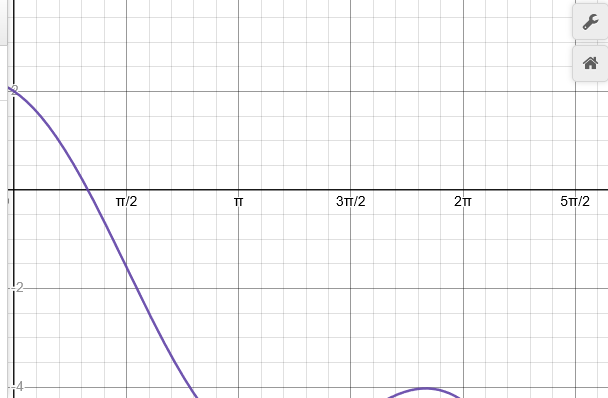
\includegraphics{38.png}

\vs\next
42.\begin{align}
    \set
    y&=2(x-2)+\cot x,\,\,0<x<\pi\\
    y'&=2-\csc^2 x=0\,\,\text{when}\,\, x=\frac{\pi}{4},\,\,\frac{3\pi}{4}\\
    y''&=2\csc^2 x\cot x=0\,\,\text{when}\,\, x=\frac{\pi}{2}
\end{align}
\begin{enumerate}
    \item Relative maximum: $\left(\frac{3\pi}{4},\,\,\frac{3pi}{2}-5\right)$
    \item Relative minimum: $\left(\frac{\pi}{4},\,\,\frac{\pi}{2}-3\right)$
    \item Inflection point: $\left(\frac{\pi}{2},\,\, \pi-4\right)$
    \item Vertical aymptotes: $x=0\,\,\pi$
\end{enumerate}
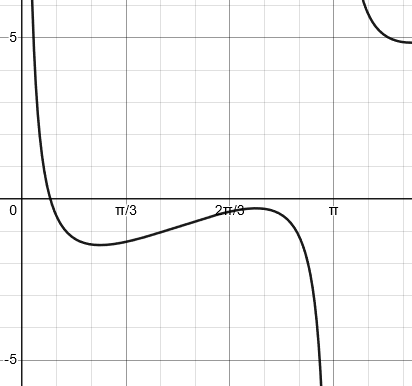
\includegraphics{42.png}

\section{The graphs of $f$, $f'$, and $f''$ are shown on the same set of coordinate axes. Which is which? Explain your reasoning.}
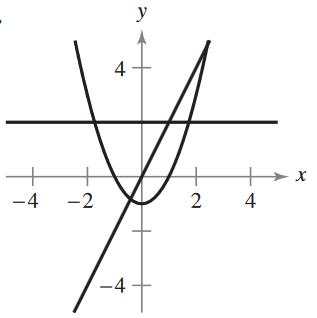
\includegraphics{50.png}\\
\begin{enumerate}
    \item $f$ is a quadratic function.
    \item $f'$ is a linear function.
    \item $f''$ is a constant function.
\end{enumerate}
The degree of the function decreases by one with each derivative, going from 2nd (quadratic) to 1st (linear) and 0th (constant).

\section{Use a graphing utility to graph the function. Use the graph to determine whether it is possible for the graph of a function to cross its horizontal asymptote. Do you think it is possible for the graph of a function to cross its vertical asymptote? Why or why not?}
\[g(x)=\frac{3x^4-5x+3}{x^4+1}\]
No vertical asymptotes and a horizontal asymptote at $y=3$. The graph crosses this asymptote, and because $f(c)$ is undefined, the graph would not cross a vertical asymptote at $x=c$.

\section{Use a graphing utility to graph the function. Explain why there is no vertical asymptote when a superficial examination of the function may indicate that there should be one.}
56.\begin{align}
    \set
    g(x)&=\frac{x^2+x-2}{x-1}\\
    &=\frac{(x+2)(x-1)}{x-1}\\
    &=
        \begin{cases}
            x+2\,\,\text{if}\,\, x\neq 1\\
            \text{undefined}\,\,\text{if}\,\, x=1
        \end{cases}
\end{align}
The rational function has a hole at (1, 3), and is not reduced to its lowest terms.

\section{Use a graphing utility to graph the function and determine the slant asymptote of the graph. Zoom out repeadetly and describe how the graph on the display appears to change. Why does this occur?}
58.\begin{align}
    \set
    g(x)&=\frac{2x^2-8x-15}{x-5}\\
    &=2x+2-\frac{5}{x-5}
\end{align}
The graph is approaching the slant asymptote $y=2x+2$.

\section{Use the graph of $f'$ to sketch a graph of $f$ and the graph of $f''$.}
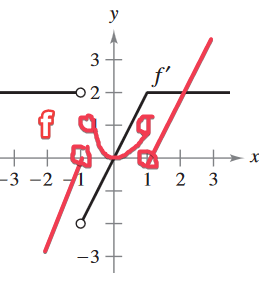
\includegraphics{64a.png}
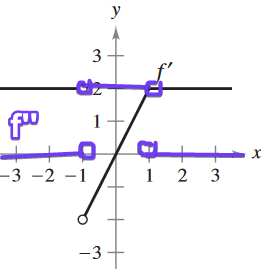
\includegraphics{64b.png}

\section{Graphical reasoning}
66. Consider the function $f(x)=\tan(\sin\pi x)$.
\begin{enumerate}[(a)]
    \item Use a graphing utility to graph the function.
    \item Identify any symmetry of the graph.
        \begin{align}
            \set
            f(-x)&=\tan(\sin(-\pi x))\\
            &=\tan(-\sin\pi x)\\
            &=-\tan(\sin\pi x)\\
            &=-f(x)
        \end{align}
        The graph is symmetric with respect to the origin.
    \item Is the function periodic? If so, what is the period?\\
        The function is periodic and a has a period of 2.
    \item Identify any extrema on (-1, 1).\\
        There is a relative maximum at $\left(\frac{1}{2},\,\,\tan 1\right)$ and a relative minimum at $(-\frac{1}{2},\,\,-\tan 1)$.
    \item Use a graphing utility to determine the concavity of the graph on (0, 1).\\
        The graph is concave downward at this point.
\end{enumerate}

\section{Create a function whose graph has the given characteristics.}
68.\begin{enumerate}
    \item Vertical asymptote: $x=-5$
    \item Horizontal asymptote: None
\end{enumerate}
\[y=\frac{x^2}{x+5}\]

\section{Capstone}
72. Identify the real numbers $x_0$, $x_1$, $x_2$, $x_3$, and $x_4$ in the figure such that each of the following is true.\\
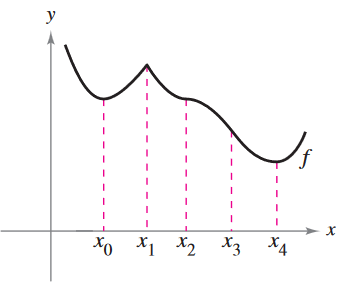
\includegraphics{72.png}
\begin{enumerate}[(a)]
    \item $f'(x)=0$\\
        This a horizontal tangent that can be identified at $x_0$, $x_2$ and $x_4$.
    \item $f''(x)=0$\\
        This is a point of inflection identified at $x_2$ and $x_3$.
    \item $f'(x)$ does not exist.\\
        This is true at $x_1$ because a sharp corner can be seen at this coordinate.
    \item $f$ has a relative maximum.\\
        It would be at $x_1$
    \item $f$ has a point of inflection.\\
        As previously mentioned in (b), these are $x_2$ and $x_3$. At these points there is a change in the graph's concavity.
\end{enumerate}








































































\end{document}